\chapter{总结与展望}

\section{全文总结}

过去几十年,定制化硬件的发展经历过高潮与低谷。十年前,在数据中心的每台服务器上添加一种定制化计算设备无异于天方夜谭。近年来,云计算规模化的趋势、数据中心应用的需求以及通用处理器的性能局限将定制化硬件的发展带上了快车道,数据中心网络的性能也一日千里。

得益于定制化硬件的发展和分布式系统的通信需求,可编程网卡在数据中心被广泛部署:微软用 FPGA 加速搜索引擎、虚拟网络、压缩、机器学习推理等,亚马逊和阿里云加速虚拟网络、虚拟存储和虚拟机监控器,腾讯云用 FPGA、华为云用网络处理器加速虚拟网络……
回望历史长河,网络虚拟化也许是可编程网卡的第一个杀手级应用,但这只是可编程网卡潜力的冰山一角。

要使应用程序充分利用数据中心网络的高性能,必须尽量降低 ``数据中心税'',这不仅包括网络虚拟化,还包括网络功能和操作系统通信原语。
本文提出用基于 FPGA 的可编程网卡加速网络功能。为了简化 FPGA 编程,本文提出首个适用于高速网络数据包处理、基于高级语言的 FPGA 编程框架,相比传统基于CPU的网络功能,吞吐量提高了 10 倍,延迟降低到 1/10。
为了降低操作系统通信原语的开销,本文提出一个软硬件结合的用户态套接字系统,与现有应用程序完全兼容,并能实现接近硬件极限的吞吐量和延迟,解决了长期以来通用协议栈性能较低、专用协议栈兼容性较差的矛盾。

``可编程网卡'' 得名于网络加速,但它不会止步于网络,会继续向系统的各个领域深入。
内存数据结构存储是分布式系统的重要基础组件。
本文提出远程直接键值访问原语,作为远程直接内存访问(RDMA)原语的扩展。通过在服务器端绕过 CPU,用可编程网卡直接访问主机内存,以及一系列性能优化,本文实现了10倍于 CPU 键值存储系统的吞吐量和微秒级的延迟,是首个单机性能达到10亿次每秒的通用键值存储系统。

毫无疑问,可编程网卡可以提高系统的性能,降低数据中心的成本。
本文提出的三个系统为虚拟网络功能、通用内存键值存储和套接字网络协议栈树立了新的性能里程碑。
但本文的目的不是打破性能记录,而是启发读者思考:如何建设包括硬件、开发工具链、操作系统在内的可编程网卡生态系统?可编程网卡等新硬件将如何改变数据中心的架构和分布式系统的编程范式?
正如有人所说,``预测未来最好的方式就是创造未来'',可编程网卡的故事才刚刚开始。

\section{未来工作展望}

基于可编程网卡的高性能数据中心系统需要软硬件结合的生态系统,主要由硬件、开发工具链和操作系统构成。
第 \ref{future:progammable_nic} 节将展望未来的可编程网卡硬件架构。
开发工具链包括编程框架、编译器、运行库、调试工具等,在软硬件协同设计中至关重要。第 \ref{future:toolchain} 节将展望开发工具链方面的几个未来工作。
操作系统包括虚拟化、调度、监控、高可用、灵活缩放等。第 \ref{future:os} 节将展望操作系统方面的未来工作。
最后,作为数据中心一等公民的可编程网卡在提高系统性能的同时,也使我们重新思考分布式系统的总体架构,可能带来系统创新,这是第 \ref{future:system} 节将讨论的。

\subsection{基于片上系统的可编程网卡}
\label{future:progammable_nic}


\begin{figure}[htbp]
	\centering
	\subfloat[本文使用的 Catapult 可编程网卡。]{
		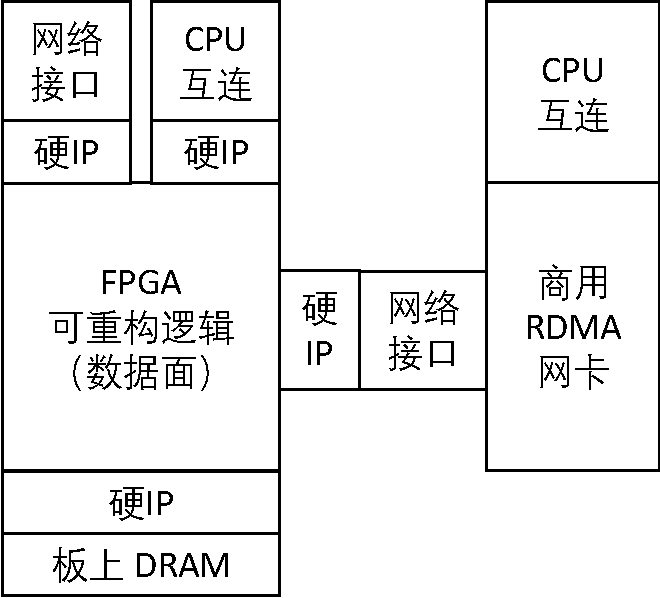
\includegraphics[width=0.4\textwidth]{figures/smartnic-current.pdf}
		\label{conclusion:fig:smartnic-current}
	}
	\hspace{0.05\textwidth}
	\subfloat[未来的片上系统。]{
		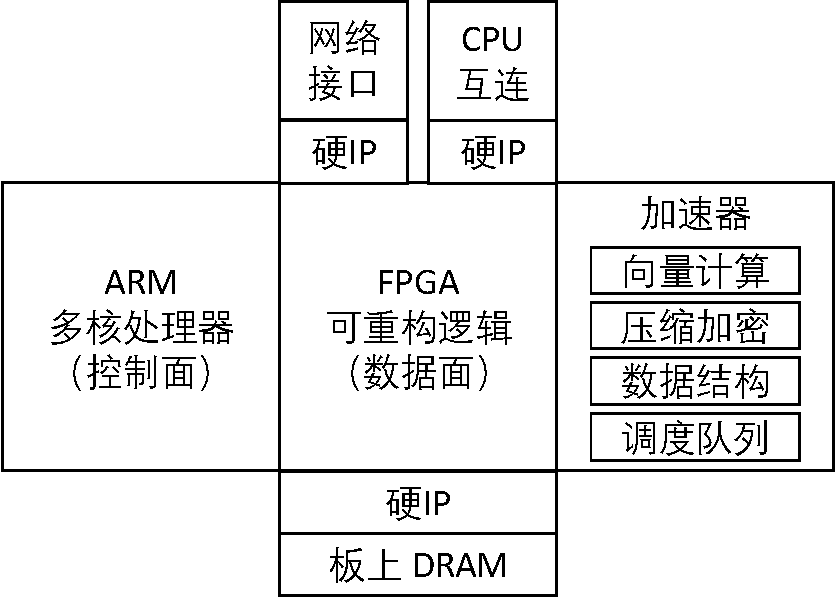
\includegraphics[width=0.5\textwidth]{figures/smartnic-soc.pdf}
		\label{conclusion:fig:smartnic-soc}
	}
	\caption{可编程网卡结构的比较。}
\end{figure}

本文使用了图 \ref{conclusion:fig:smartnic-current} 所示的 Catapult 可编程网卡。这种架构有三个局限性。
首先,现有的商用 RDMA 网卡当并发连接数较多时,性能会急剧下降 \cite{mprdma}。我们希望利用第 \ref{chapter:kvdirect} 章可扩放键值存储的技术,在 FPGA 可重构逻辑中实现 RDMA 硬件传输协议,实现高并发连接数下的高性能。这已经在第 \ref{socksdirect:sec:discussion} 节讨论过。
其次,FPGA 只适合加速数据面,控制面仍然留在主机 CPU 上。尽管它的计算量不大,但为了性能隔离,计算节点仍然需要预留少量 CPU 核用于控制面处理。第 \ref{chapter:intro} 章已经指出,即使预留一个物理 CPU 核也是相当昂贵的。为此,我们希望在可编程网卡中加入 ARM 多核处理器,用于实现控制面,从而完全消除主机 CPU 上的虚拟化开销。ARM 多核处理器的成本为数十美元,远低于一个物理 CPU 核的成本。
最后,一些类型的工作负载在 FPGA 内实现的效率不是很高,应当固化在 ASIC 加速器中。第一类是深度学习和机器学习中的向量操作、加密解密操作等计算密集型操作。例如,Intel QuickAssist 加速卡 \cite{intel-qat} 基于 ASIC 的 RSA 非对称加密比第 \ref{chapter:clicknp} 章基于 FPGA 的实现,吞吐量约高 10 倍;基于 ASIC 的 LZ77 压缩算法比本文基于 FPGA 的实现,吞吐量也高一个数量级。所用 ASIC 和 FPGA 芯片的功耗、面积和制程都接近。
第二类是常见数据结构和调度队列。基于内容寻址内存(Content-Addressable Memory,CAM)的查找表是哈希表、乱序执行引擎、缓存、模糊匹配表等多种常见数据结构的必要组件。CAM 在 ASIC 中可以用三态门实现,而在 FPGA 中实现的效率较低 \cite{wong2011comparing}。
此外,优先队列(可用移位寄存器序列或堆实现)、轮转(round-robin)调度队列、考虑依赖关系的乱序执行调度器、定时器等结构在很多应用中广泛使用,从而可以借鉴网络处理器(Network Processor)的架构,将这些通用结构硬化,让 FPGA 可重构逻辑专注于定制化计算和灵活互连。

因此,本文期待未来的可编程网卡使用如图 \ref{conclusion:fig:smartnic-soc} 所示的片上系统架构。
相比使用片外总线互连的分离组件,片上系统可以使组件间通信的带宽更高、延迟更低,更适合将计算细粒度地拆分到更适合的处理组件。
位于片上系统中心的 FPGA 不仅提供了可编程性和计算能力,也可以灵活互连和组合片上的各种计算加速器,组建定制化的内存层次结构,还可以灵活互连主机内外的各种硬件设备,组成数据中心智能互连(intelligent fabric)。

目前,业界已有基于片上系统的可编程网卡架构。例如,Xilinx 的 Versal 架构 \cite{vissers2018keynote,vissers2019versal,gaide2019xilinx} 将可重构硬件(FPGA),基于超长指令字(VLIW)的深度学习和传统机器学习加速器、数字信号处理器(DSP)和硬核(hard IP),以及多核通用处理器集成在一块芯片上,组成片上系统(System on Chip)。与传统 FPGA 相比,Versal 架构最大的区别是组成了片上系统,体现在三方面:第一,把内存控制器、PCIe 等外部接口的控制逻辑从可重构逻辑硬化成数字逻辑,减少了 FPGA 面积的开销,还能使 FPGA 实现即插即用。第二,认识到向量操作等大数据、机器学习常见计算在 FPGA 上实现的较低效率,并使用硬化的数字逻辑进行加速。第三,增加了通用处理器,可以处理复杂逻辑和控制平面,而无需绕回 CPU,这使得 Versal 片上系统可以直接驱动 Flash 存储等,组成低成本的存储服务器,而无需传统的 x86 CPU 等组件。片上系统的部件之间通过片上网络互连 \cite{swarbrick2019network,gaide2019xilinx}。Versal 架构针对数据中心服务器的多种应用加速,开发者可以把应用分解成通用处理器上的控制面、可重构硬件数据面、向量计算数据面,用合适的体系结构处理应用中的相应部分。



\subsection{开发工具链}
\label{future:toolchain}

目前,可编程网卡是主要由云计算厂商推动的新兴事物,其生态系统还不够完善。
首先,可编程网卡的编译器、调试工具、代码库等开发工具链不够灵活和易用,相关厂商的支持也不够完善。
近年来的高层次综合工具主要关注 FPGA 在计算密集型处理(如深度学习)方面的可编程性,而对通信密集型处理的关注较少。
尽管本文第 \ref{chapter:clicknp} 章的 ClickNP 在此方向做了一些努力,但与规模化的商业应用还有较大距离。

其次,目前的研究中,可编程网卡与应用程序间的任务划分是较为随意(ad-hoc)的,需要量化研究方法来确定哪些工作负载适合卸载到可编程网卡。
对于一个现有应用程序,要利用可编程网卡加速其数据面功能,需要重写大量代码:不仅需要在可编程网卡内从头实现数据面的处理逻辑,还需要修改主机 CPU 上的控制面代码以充分利用网卡的并行性和隐藏处理延迟。未来的开发工具链需要降低现有应用的二次开发成本。


\subsubsection{基于可编程网卡的 PCIe 调试工具}
\label{future:pcie-debugger}

数据中心服务器承载着越来越多的 PCIe 设备,如 GPU、NVMe SSD、网卡、加速卡和 FPGA 等。为了 PCIe 设备之间高吞吐量和低延迟的通信,GPU-Direct、NVMe over Fabrics 等技术开始流行。然而,很多 PCIe 设备只能跟 CPU 上的设备驱动程序通信,其 PCIe 寄存器和 DMA 接口很复杂,且可能没有文档。为了在 PCIe 上抓包和调试 PCIe 协议的实现,开发者往往需要昂贵的 物理层 PCIe 协议分析仪(价值 25 万美元左右)。协议分析仪需要实验室环境,难以在生产环境中动态调试。而且,协议分析仪无法修改 PCIe 数据包,也没有足够的可编程性来从大量的流量数据中发现异常或统计规律。

一个未来的方向是基于可编程网卡实现透明 PCIe 传输层协议(TLP)调试器。PCIe 调试器抓取 PCIe 设备和 CPU 之间的通信数据包。
这项工作的挑战在于,由于 PCIe 的物理拓扑和路由是固定的,不可能在 PCIe 上实施与局域网中的 ARP 类似的攻击。
然而,通过欺骗设备驱动程序,PCIe 流量可以被重定向到 PCIe 调试器。
根据请求的发起方,把 PCIe 和 CPU 之间的通信分成两类。

第一类是 CPU 发起的内存映射 I/O(MMIO)操作。这类操作中,CPU 访问 PCIe 基址寄存器(BAR)指向的内存区域。驱动程序从操作系统内核例程中获得 BAR 地址,因此可以修改该操作系统内核例程,返回 PCIe 调试器的地址,而非设备本身的地址。然后在 PCIe 调试器中建立地址映射,使 CPU 的内存映射 I/O 操作传输到 PCIe 调试器,PCIe 调试器作为代理再把请求发送给目标设备。

第二类是设备发起的 DMA 操作,用以访问主机内存。表面上看来,没有办法预知设备会访问哪个内存地址。然而,良定义的设备应当只访问驱动程序分配给该设备的地址。在 Linux 中,有两种设备驱动程序获取可 DMA 内存区域及其物理地址的方法。计划对这两种操作系统例程分别加以修改,在分配 DMA 内存区域时用 PCIe 调试器的地址取代主机内存地址,并建立 PCIe 调试器中的地址映射。这样,当设备试图 DMA 到主机内存时,事实上是 DMA 到了 PCIe 调试器,调试器随后根据映射表把数据再 DMA 到主机内存。

通过这种方法,主机驱动程序和 PCIe 设备的通信都将被 PCIe 调试器截获。基于 FPGA 的 PCIe 传输层协议调试器有足够的灵活性来修改、统计、过滤和注入数据包,进而实现对 PCIe 设备的模糊测试(fuzz testing)和压力测试。


\subsubsection{微秒级延迟隐藏}
\label{future:latency-hiding}

使用定制化硬件加速应用程序上的 CPU 处理时,原有的 CPU 软件处理逻辑被替换成了向加速器发送命令、等待加速器处理和从加速器接收结果三个步骤。在等待加速器处理期间,CPU 线程被阻塞。类似地,在分布式系统中,经常需要进行远程过程调用(RPC)并等待其他微服务或节点返回结果。传统上,开发者一般采用增加更多线程的方式隐藏加速器处理和远程过程调用延迟,也就是让操作系统在此期间切换到其他线程进行处理。然而,随着数据中心加速器性能的提高和加速任务粒度的降低,一些加速任务的执行时间只有数微秒至数十微秒。类似地,远程过程调用的网络延迟也从之前的数毫秒降低到数微秒至数十微秒。操作系统切换线程调度也需要 3 至 5 微秒,几乎与加速任务的执行时间和远程过程调用的网络延迟相当。这就意味着在等待期间切换到其他线程并不经济,让 CPU 在当前线程上等待加速任务完成可能是更好的做法。但是,这也就意味着等待期间 CPU 时间的浪费,在一定程度上影响了定制化硬件加速器节约 CPU 的效果。

一个未来研究方向是从编译的角度出发,实现应用程序的微秒级延迟隐藏。
我们有两个主要的观察:首先,应用程序可能有多个互相不依赖的硬件加速任务需要处理,因此可能挖掘出这些不依赖的加速任务,进行并发处理。
其次,很多应用程序是事件驱动的,也就是在一个永久循环里依次处理到来的事件。不同的事件处理之间可能没有依赖关系,这时就可以暂时挂起正在被处理的事件,去处理下一个不相关的事件。

这两种延迟隐藏方案的困难在于 ``依赖关系'' 的判断。在函数式编程语言中,纯函数之间的依赖关系比较容易判断。但在大多数开发者通常使用的编程语言中,内存是共享的,很多代码之间都存在依赖。例如,创建对象时需要分配内存,影响内存布局,因此从严格意义上讲,任意两个对象的创建顺序都是有依赖的。再如,两个远程过程调用是否存在依赖,往往取决于其语义。因此,问题的核心挑战是由开发者指明哪些依赖事实上是不必要的。

一种可能的方案是 ``async'' 修饰器,允许开发者指定一个函数可以被异步执行。async 函数内部可以使用 wait 调用来注册事件、释放 CPU 并在事件成立时唤醒(例如等待加速器或远程过程调用的返回)。可被异步执行的函数执行过程中不会被打断(除非调用了 wait,或有可被异步执行的子例程),因此不必担心可重入问题。每个 async 函数的执行用协程(coroutine)实现。进一步地,提出 ``async pure'' 修饰器,允许开发者指定一个函数不仅可以被异步执行,还没有任何副作用,这样就可以推测执行,即在执行的条件尚未确定时就执行之,而无需担心其产生不可撤回的副作用。

例如,把无状态计算卸载到加速器、只读的远程过程调用、打开文件是 async pure 函数。而执行写操作的远程过程调用、处理一个事件的例程是一般的 async 函数。如果 async 函数之间存在逻辑依赖关系,例如同一个用户发起的不同事件需要按顺序依次处理,那么可以为每个用户设置一个锁,在事件处理开始时加锁并在结束后解锁。锁使用 wait 调用实现,因此开销很小。

除了从编译的角度挖掘应用程序内部的并行性,另一个未来研究方向是从体系结构的角度出发,实现硬件管理的高性能上下文切换和调度 \cite{barroso2017attack}。第 \ref{smartnic-np} 节介绍的网络处理器硬件调度器可以作为有益的借鉴。

\iffalse
\subsubsection{高级语言到低级语言的翻译}
\label{future:high-to-low}

现代软件享受着摩尔定律的红利,为了开发效率,一般使用高级语言模块化编程,而编译器对软件的优化并不充分。高级语言编写的现代软件,即使与多年前基于底层语言(如 C 语言)的软件功能相似,其性能往往也相差很多。``安迪-比尔定律'' \cite{langchaozhidian} 形象地刻画了这种现象,即高性能的新型处理器(以 Intel 的 CEO 安迪代表)所增加的性能,往往被软件(以微软的创始人比尔·盖茨代表)所消耗,最终用户感受到的性能仍然是相似的。从编程框架、编译器等角度优化软件的性能也有很大的空间。David Patterson 指出,把 Python 语言重写为 C 语言,应用程序的性能可以提高 50 倍,而如果使用一系列优化,实现 1000 倍于 Python 的性能提升并不是梦想 \cite{python-to-c}。

未来的研究方向是从高级语言到低级语言的自动翻译。尽管很多高级语言是动态类型的,还有自省等高级语言特性,但对一个给定的高级语言应用程序,其输入的类型往往是相对确定的。
\fi

\subsubsection{网络应用数据面自动生成}
\label{future:p4coder}

为了提升网络应用的性能、降低 CPU 开销,数据中心引入了可编程交换机和网卡以卸载虚拟化网络功能、传输协议、键值存储、分布式一致性协议等。与通用处理器相比,可编程交换机和可编程网卡的资源较少,支持的编程模型也较为受限。
为此,开发者通常把一个网络功能分割成处理通常情况数据包的数据面和处理其余情况的控制面。数据面功能在一个数据包处理语言(如 P4)中实现,并卸载到硬件。

为网络应用卸载而编写数据包处理程序需要很多劳动。首先,即使拥有协议说明书或源代码,开发者仍然需要阅读上千页的文档或代码,进而发现哪一部分是常用功能。其次,很多实现与协议说明书之间存在细微的区别,因而开发者经常需要检查数据包的抓包记录,手工反向工程出特定于一个实现的行为。

未来的研究方向是自动学习指定网络应用的行为,从而自动生成数据面参考代码。
这样,开发者只需设计一些简单的数据面的测试用例,并运行指定的网络应用。
数据面自动生成系统将捕获输入和输出的数据包,并搜索一个数据包程序来对指定的输入测试用例产生测试得到的输出。
显然,通过测试用例并不意味着程序能在其他输入的情况下正确地泛化,因此自动生成的代码只能作为开发者的参考,开发者可以在其基础上补充特殊情况处理的细节。尽管如此,自动生成的参考程序可以帮助开发者理解协议在通常情况下的工作方式,节约大量开发时间。


一般意义上,通过例子生成程序被认为是困难的,由于巨大的搜索空间和理论上不可判定的停机问题。幸运的是,可以被卸载到硬件的数据包程序通常是比较简单的。商用可编程交换机和网卡并不支持循环和递归,因此不存在停机问题的判定难题。此外,对于每个持久化状态,每个数据包在数据面上只允许一次读写操作。而且,从数据包输入到输出的逻辑深度被硬件的流水线深度所限制。这些限制极大地降低了程序的搜索空间。
更重要的是,为了减小搜索空间,可以主动生成测试用例,以消除一些可能的搜索方向。
为了尽可能泛化测试用例,使用生成测试(generate and test)的方法来观察指定应用的行为。为了在可能的无穷多种可以生成指定输出的程序中选定一种,使用奥卡姆剃刀准则,选择具有最小描述长度的程序。当存在多个描述长度相同的程序时,系统可以生成判定性测试用例来决定正确的那个,或者报告用户。

\subsubsection{异构分布式系统的任务划分}
\label{future:work-split}

数据中心是一个异构硬件组成的分布式系统。每种硬件有一定的计算、存储和网络互连资源。不同硬件能够进行的计算类型和计算效率都不同,例如 CPU 适合控制密集型的计算,GPU 适合一般的单指令流多数据流(SIMD)类型计算,TPU 适合卷积和矩阵乘法类计算,FPGA 适合通信密集型计算。异构的硬件之间通信的能力也不同,例如 GPU 之间可以通过 NVLink 直接通信,而作为可编程网卡的 FPGA 是服务器主机与数据中心网络之间的必经之路。

给定一个计算流图及其中每个元件的高层次语言描述,一个重要的问题是如何把元件映射到异构的计算硬件。显然,仅仅考虑每个元件在各种计算硬件上的执行效率是不够的,还需要考虑元件之间通信的开销。例如,神经网络中卷积层之间的归一化运算可能在 GPU 上执行效率高于 TPU,但 GPU 和 TPU 之间数据搬移的开销可能超过在 TPU 上执行归一化运算的性能损失,因此在 TPU 上融合卷积和归一化运算可能是性能更优的。

一般地,可以将异构计算集群形式化为一张拓扑图,图中的顶点是计算设备、内存和存储设备和网络交换设备,边是节点间的数据通路。每个计算设备有若干支持的计算类型和各类型计算的带宽和延迟,而数据通路的属性包括带宽、延迟。计算流图中的每个顶点表示计算量和计算类型,每条边表示所需传输的数据量。任务划分问题的目标就是找到计算流图到异构计算集群拓扑图的一个映射,使得延迟、吞吐量满足应用的约束。

对于计算规模大的元件,还需要拆分到多个硬件上并行执行或流水线执行。一个元件的计算可能有多种拆分方式,不同拆分方式所需的通信开销不同。需要根据系统性能需求或异构硬件数量的限制计算出每个硬件上所需执行的计算量,然后根据通信和计算开销模型得到优化的元件拆分方案。



\subsection{操作系统}
\label{future:os}

分布式系统的 ``操作系统'' 包括主机上的传统操作系统和分布式系统的调度、管理、监控系统及共享的基础服务中间件。
本文研究了操作系统网络协议栈和分布式系统键值存储的优化,但操作系统中还有存储等多个子系统,分布式系统中也有消息队列等多种中间件。这些子系统和中间件显然也可以用可编程网卡加速。

此外,在传统分布式系统中,由于通信成本较高,热迁移和高可用往往需要开发者使用特定的编程框架。在拥有高性能数据中心网络的数据中心,基于可编程网卡,将可能实现通用应用程序的高效热迁移和高可用。这将让数据中心更像是一台巨大的计算机,应用可以充分利用异构的计算、存储资源,且几乎不可感知硬件故障。

\subsubsection{存储虚拟化加速}
\label{future:storage-virtualization}

云计算中的虚拟存储由本地存储和远程存储两部分构成。
远程存储则是由存储节点虚拟出的分布式存储系统,提供高可靠性、高可用性、容量可扩放性和吞吐量可扩放性,是云平台中的主要存储方式。
本地存储包括非易失性内存(Non-Volatile Memory,NVM)和 NVMe 高速闪存盘(flash storage),主要用于需要极致性能,但数据不需要高可靠性存储的分布式数据库等应用。

虚拟存储提供给客户的最基本服务是块存储(block storage),可以作为块设备(block device)挂载到虚拟机作为磁盘使用。
云服务还提供了对象存储(object storage)、文件存储(file storage)等存储服务。
这类服务大多提供类似键-值(key-value)映射的抽象,即用户指定键,读取(GET)或写入(PUT)相应的值。
键-值存储作为一种基础数据结构,可以分为持久化存储、临时存储;根据是否需要复制和容灾,是否支持事务(transaction),提供强一致性或最终一致性 \cite{anna},是否支持范围索引、二级索引、内容索引等,可以组合出形形色色的存储系统,满足不同应用的需求。

虚拟存储系统的两个基本逻辑概念是客户端和服务器。
如图 \ref{background:fig:storage_arch} 所示,客户端是云存储服务的使用者,如云上承载客户虚拟机的计算节点;服务器提供块存储、对象存储、文件存储等抽象,把逻辑存储的读写请求映射到物理存储介质的读写请求。
多个客户端可能共享同一个虚拟存储,例如分布式数据处理系统中的多个计算节点可能需要访问共享的原始数据和配置参数,数据处理的中间结果也可以通过存储来传递。
同一个虚拟存储可能对应多个存储服务器,用于实现存储的容量可扩放性、吞吐量可扩放性、容错和高可用。


\begin{figure}[htbp]
	\centering
	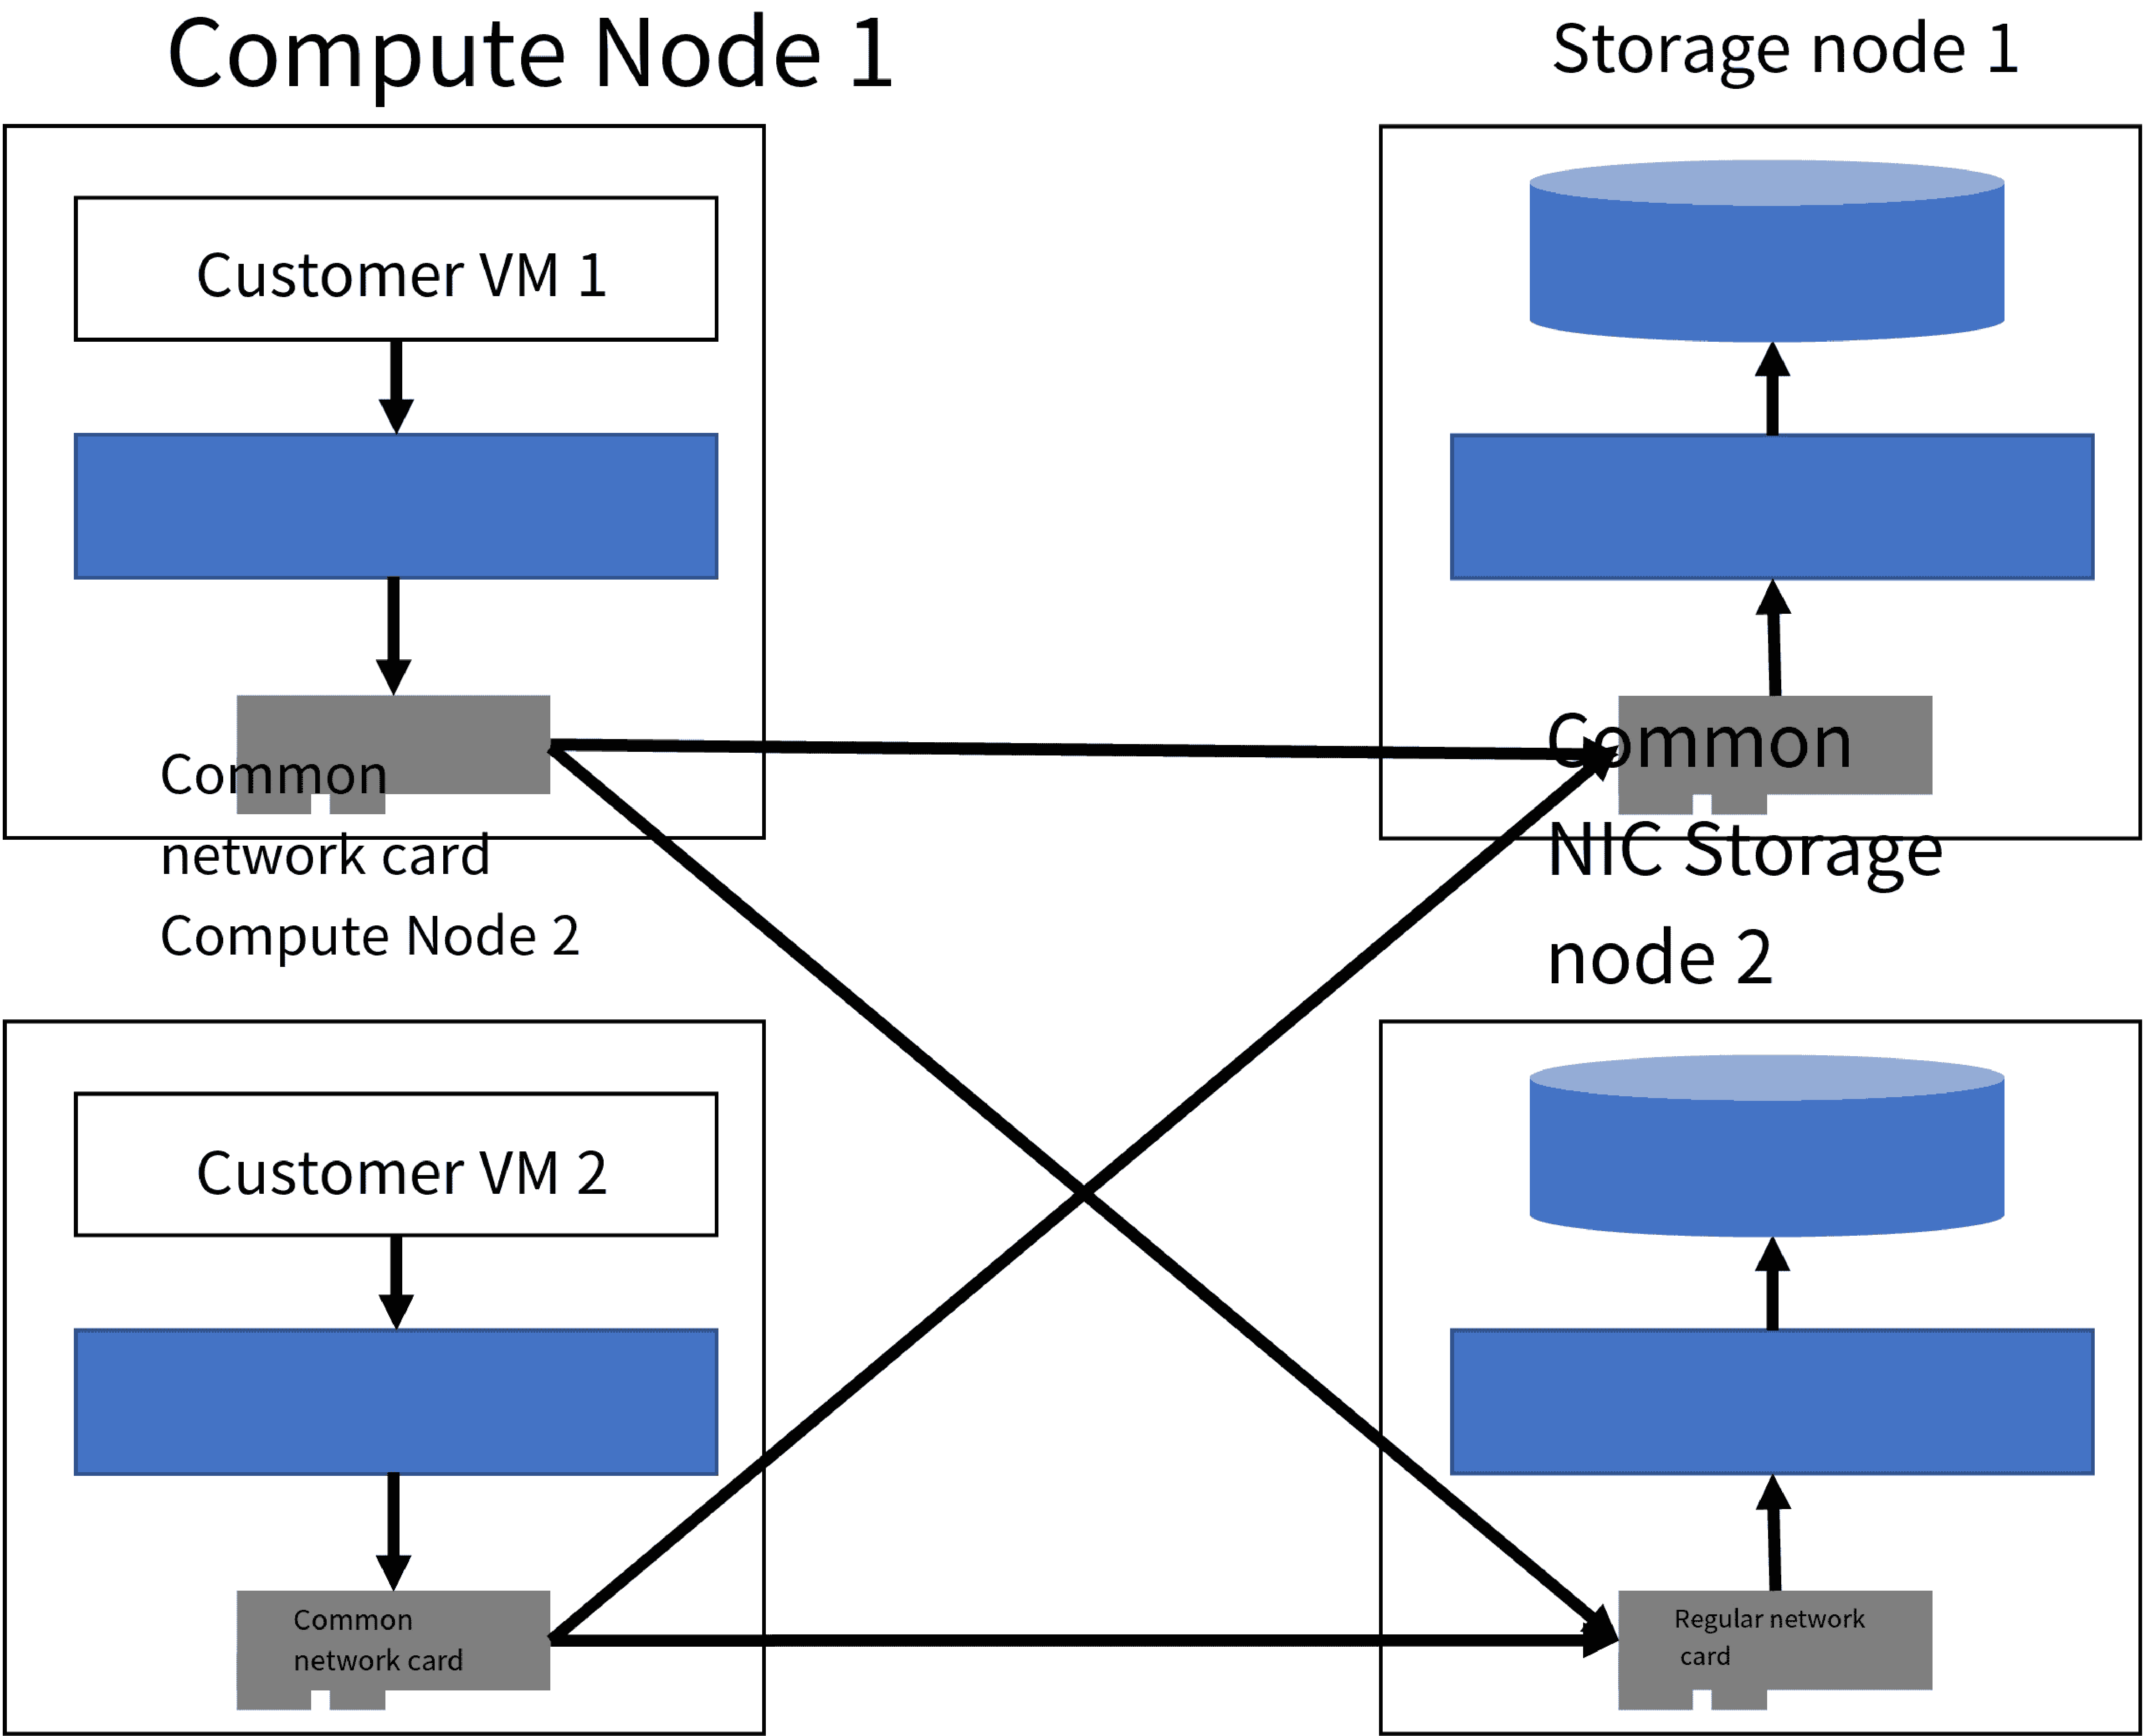
\includegraphics[width=0.6\textwidth]{figures/storage_arch.pdf}
	\caption{数据中心云存储的简要架构。}
	\label{background:fig:storage_arch}
\end{figure}


上述存储服务器的结构是较为简化的,事实上往往分为多个层次。
例如,微软 Azure 的云存储服务分为前端节点、中间节点和后端节点 \cite{calder2011windows}。
前端节点负责解析和验证请求,并根据数据分片映射表(例如键的哈希值),分发到数据所在分片的中间节点。中间节点负责实现请求的处理和存储数据结构的处理,把用户的请求映射成一系列存储读写操作,分发给对应的后端节点。后端节点负责实现数据的复制(replication)以及在物理介质上的存储。

在软件处理之外,数据中心存储还有显著的网络开销。
在数据中心中,由于存储服务器需要安装较大容量的存储介质,存储节点的硬件配置一般与计算节点是不同的。此外,计算节点上由于运行客户的虚拟机,虚拟机监控器软件经常需要升级以增加新功能和修补安全漏洞,因此计算节点的稳定性通常比存储节点低。为了保证存储的高可用性,存储节点与计算节点通常是分离在不同物理主机上的。因此,计算节点上的存储客户端通常需要把数据从存储服务器通过网络搬运过来。
也就是说,客户虚拟机的每个 I/O 请求都需要被虚拟机监控器捕获,然后从计算节点上虚拟机监控器内的存储客户端软件出发,依次经过存储服务器的前端、中间和后端节点的处理,才能到达存储介质。
为了保证数据的安全性,物理存储介质上的数据一般需要加密存储。为了节约存储空间,降低单位存储容量的存储介质成本,很多云厂商还会对存储的内容进行压缩。压缩和加密一般在存储服务器上进行,属于计算密集型操作。例如,根据实验,在 LZ77 较好的压缩率下,一个服务器 CPU 核心每秒通常只能压缩 100 MB 的数据;对 1 KB 的块,AES 加密和 SHA-256 签名每秒也只能处理 100 MB 的数据。

由于软件处理和网络传输的开销,云计算平台上块存储的延迟一般为 0.5 至 1 毫秒,对象存储的延迟一般为 1 至 10 毫秒 \cite{jonas2019cloud},远高于物理存储介质的延迟(如 SSD 的延迟一般为 0.1 毫秒)。
此外,云存储的吞吐量也低于相应的物理存储介质,例如 SSD 云盘最高的吞吐量为 50 K 次 I/O 每秒,而单块数据中心级 SSD 的吞吐量就已达数百 K 次 I/O 每秒 \cite{jonas2019cloud}。
为了充分利用最新的数据中心存储硬件的性能,云存储服务需要全栈优化。
例如,很多数据中心在存储协议栈的网络传输方面,已经使用 RDMA 协议降低了网络协议栈的 CPU 开销和延迟 \cite{guo2016rdma}。
一些数据中心还通过改进云存储的协议栈,把客户端、服务器前端、中间、后端节点的功能进行适当的整合,减少层次 \cite{nitro-blog}。
HyperLoop \cite{kim2018hyperloop} 利用 RDMA 网卡和非易失性内存(NVM)降低了存储写入事务的延迟。

\subsubsection{远程过程调用和消息队列加速}
\label{future:rpc}

分布式系统中的消息传递通常采用远程过程调用(RPC)或消息队列(message queue)模型,或者两者的结合。在 RPC 模型中,服务器端注册一个过程(procedure)来响应客户端的 RPC 请求。在消息队列模型中,生产者将消息广播或者分发到若干消费者。为了实现生产者与消费者的解耦以及消息的缓冲和可靠投递,消息队列模型往往引入一个经纪人(broker)服务,如 Kafka \cite{kreps2011kafka}。在编程接口方面,分布式应用程序通常使用 RPC 库和消息队列中间件(middleware),这些库和中间件则依赖操作系统的套接字(socket)接口来发送和接收消息。
本文研究了操作系统套接字接口的加速,但没有考虑更上层的 RPC 和消息队列中间件。谷歌的研究 \cite{barroso2017attack} 表明,这些消息中间件经常增加数十微秒的延迟,占到整个端到端网络延迟的很大一部分。
为了降低分布式系统的端到端消息传递延迟,有必要利用可编程网卡等硬件和用户态库等软件,实现高性能的 RPC 和消息队列。
一种方案是在本文第 \ref{chapter:socksdirect} 章的用户态套接字系统基础上,实现 RPC 和消息队列等高层抽象;另一种方案是打破传统网络协议栈边界的全栈优化,如最近的 eRPC \cite{kalia2018datacenter} 是这方面很有意义的探索。
对于消息队列等比较简单的应用,甚至可以探索在可编程网卡中实现,绕过主机CPU。

\subsubsection{基于微内核的用户态操作系统}
\label{future:user-space-os}

本文第 \ref{chapter:socksdirect} 章提出了一个用户态网络协议栈 SocksDirect。第 \ref{chapter:socksdirect} 章的技术可以用于加速操作系统的更多抽象。

在网络协议栈之外,操作系统的存储协议栈也有较高的开销。
Linux 存储协议栈逻辑上由五层构成。首先,是与网络协议栈类似的虚拟文件系统层,提供基于文件描述符的 API。
其次,文件系统层实现文件系统的抽象,提供文件的路径查找、权限管理、空间分配等功能。
第三,缓存缓冲层与 Linux 的内存管理机制紧密结合,负责管理读缓存和写缓冲,以及页面换入换出机制。
第四,块设备层把存储设备抽象为若干个 ``块''(block),实现块访问的合并、排序等。
第五,在设备驱动层,存储介质驱动程序与硬件通信以读取和写入硬盘块。
在存储协议栈中,虚拟文件系统层也是开销的重要来源。对数据库等很多使用直接 I/O 的应用,文件系统、缓存缓冲层是不必要的。
与网络协议栈类似,存储协议栈中也存在多次数据拷贝。对于很多应用,还存在存储和网络协议栈间的拷贝。基于页面重映射的零拷贝技术可以用于网络和存储协议栈,实现每份数据在物理内存中只有一份拷贝,在协议栈间复制的仅是虚拟内存的映射关系。

本文第 \ref{chapter:socksdirect} 章的技术有更广阔的应用前景:基于微内核的用户态操作系统。
操作系统主要包括三方面的功能:资源虚拟化、进程间通信和高层次抽象。
第 \ref{chapter:socksdirect} 章实现了网络资源的虚拟化和进程间的消息传递,提供了套接字的高层次抽象。
用户态存储协议栈可以实现存储资源的虚拟化和文件系统的高层次抽象。
其余的操作系统功能还包括计算资源虚拟化(即进程调度)和进程间同步(如锁和信号量)。
这些功能可以在用户态守护进程中实现,也可以在可编程网卡中实现。
将传统操作系统的功能被移动到用户态和可编程网卡后,就可以采用微内核,并保持与现有应用程序的兼容性。

基于微内核的操作系统不仅具有更高的性能,还便于实现通用分布式应用的高可用性,这将是下一小节讨论的主题。

\subsubsection{通用分布式应用的高可用性}
\label{future:ftlinux}

硬件故障和操作系统崩溃都可能导致分布式应用的部分节点出错。
分布式应用的高可用性是很重要的。
很多现有的请求处理和批量处理系统可以简化分布式应用的容错编程。
这些程序通常需要程序员把组昂泰显式地从计算中分离,并把状态存储到一个容错存储系统中。
然而,很多现有应用(如 Node.js,Memcached 和 Tensorflow 中的 Python 逻辑)并不原生支持容错。此外,容错编程框架通常比不容错的版本性能低。
我们希望解决通用分布式应用程序的透明和高效容错的挑战。
具体来说,挑战分为进程迁移、确定性重放和分布式快照三个方面。

首先,在不同层次上的容错存在着权衡。
在体系结构层次上的容错需要定制化硬件。
在虚拟机层次上的容错机制认为所有网络通信都是双向的(因为有数据传输和 ACK 确认报文),并且不能发现诸如进程间通信的高层次语义。
系统调用层次上的容错需要对操作系统内核的修改以实现进程迁移,例如,从源主机把进程状态提取出来,并注入到目的主机里。
Linux 系统中的进程迁移较为复杂,因为来自不同进程的状态混杂在一个宏内核中。
而 Unikernel 方法不能支持很多现有的进程间通信机制。
为此,未来的研究工作可以借鉴本文第 \ref{chapter:socksdirect} 章的 SocksDirect 架构,设计一个分布式的用户态运行库操作系统,与现有 Linux 应用程序编程接口兼容。
进程的内存快照同时获得了运行库和应用程序的状态,同时保留了高层语义,便于优化。

第二,状态机复制(State Machine Replication,SMR)和快照重放(snapshot replay)是实现容错的两种主要方法。 SMR 至少需要两台主机才能执行完全相同的应用程序,从而引入 CPU 开销。基于快照的系统通常在两个相邻快照之间的间隔期间缓冲应用程序的输出,因为当主机发生故障时,系统无法保证自上次快照以来的确定性执行。这种所谓的输出提交(output commit)问题为透明容错系统引入了显着的请求服务延迟。或者,记录应用程序的所有非确定性事件仍然会产生很大的开销。未来的研究方向是采用根据其最近的执行历史来预测应用程序的非确定性事件。如果预测正确,则应用程序继续。否则,等待很短的时间来实现预测,因为许多不确定性源于微小的时间波动。这样,系统只需在等待超时的时候记录错误预测的事件,减少记录开销。

第三,透明容错机制需要在不暂停整个系统的情况下拍摄分布式应用程序的快照。一致的快照算法要求所有主机以相同的速度拍摄快照,并在任何主机发生故障时同时回滚。这种全局同步的行为与容错的目标相矛盾,容错需要系统在主机发生故障时继续提供对延迟敏感的请求。如何异步地对分布式系统生成一致的快照是未来的研究方向。


\subsubsection{基于热迁移的数据中心资源打包}
\label{future:resource-packing}

现代数据中心的资源利用率较低,有较大的优化空间。例如,数据中心内大部分物理服务器的平均使用率只有大约 10\% 到 15\%,但是闲置时的功耗却与使用率最高时相差仅 30\% \cite{barroso2018datacenter}。一方面,服务器和硬件的节能设计可以改进,以在使用率较低甚至闲置时尽量降低功耗。另一方面,云计算的一项优势就是支持热迁移,理论上可以在客户几乎不感知的情况下,根据虚拟机的计算、内存、存储、网络等需求,把需求互补的虚拟机打包安排在一台物理服务器主机上,从而最大化利用物理服务器的各种硬件资源。目前,热迁移对客户服务会造成一段时间的性能下降甚至中断,因此在云计算中的利用还不够广泛。

热迁移的主要难点在于生成一致的虚拟机状态快照。在异构硬件组成的数据中心,虚拟机的状态不仅包括其 CPU、内存和本地存储的状态,还包括 GPU、网卡等硬件的状态。这些硬件往往没有提供高效的快照和恢复功能,从而只能在新物理节点上重新加载硬件驱动程序、初始化硬件内部状态,带来较高的延迟。第 \ref{chapter:clicknp} 章的 ClickNP 框架可以实现网络元件内部状态的快照和迁移,因此采用 ClickNP 框架编写的可编程网卡可以高效热迁移。GPU-Direct RDMA 等技术可以实现 GPU 内部存储的高效传输。对于本地存储,可以利用存储解聚的思想,不必等待数据迁移完成,而可以在迁移过程中把新节点上虚拟机的访问请求重定向到原有存储。

\subsubsection{端云融合的分布式操作系统}
\label{future:distributed-linux}

智能终端(如智能手机和 PC)和云(数据中心)是目前最重要的两类计算和存储设备。端和云的计算和存储能力都在快速增长,且随着 5G 技术的发展,端云之间的通信成本将大幅降低,带宽和延迟也将显著改善。因此,端云融合将成为重要的趋势。一方面,端上的应用将可以更细粒度地调用云上的服务、访问云上的数据;另一方面,云上用于高性能通信和计算的技术也会逐渐应用到端上。例如,通过在端上部署可编程网卡,可以为 5G 网络通信降低功耗开销,消除性能瓶颈;可以提高访问 Flash 存储的性能,本文第 \ref{chapter:socksdirect} 章的高性能用户态套接字技术也可以在端上得到应用。

当端上的应用需要较大的算力、存储空间,或需要长时间地运行任务时,往往需要卸载到云上处理。无服务器计算(serverless computing)简化了云上的任务调度,但仍然需要开发者在端云间进行任务划分,并设计远程过程调用(RPC)接口。
本文期待未来的工作提出端云融合的分布式操作系统。在端云融合操作系统中,应用在端和云上有相同的开发环境和运行环境。应用可以直接访问云上的计算、存储和网络资源,而无需关注其本身是运行在端上还是云上。
一个应用由若干进程组成,每个进程运行在端或云上的一个计算设备上,并允许动态迁移计算设备;不同进程可以运行在不同的计算设备上,进程间可通过分布式操作系统提供的基于消息传递或共享数据结构存储的中间件来通信。
为了支持网络测量、爬虫等需要分布在不同地理位置的应用、由于隐私保护法律需要限制数据的处理和存储区域的应用以及为了开发者提升数据局部性,应用可以指定进程可以运行、数据可以存储的计算设备集合。
分布式操作系统的主要挑战是将进程内存状态和共享数据结构存储中的数据在端云的计算节点之间合理复制和缓存,以提高数据局部性,降低通信延迟。

作为一个示例,用户在 PC 终端上启动一个并行编译任务,传统上该任务的并行度将受限于 PC 上的 CPU 核数,且消耗 PC 较多的电池能量。在端云融合的分布式系统中,如果传输源文件及编译结果的通信代价低于计算的代价(或者待编译文件在云上已经有副本),该任务将被分发到云端的多台服务器上,编译任务的不同子进程将运行在不同服务器的 CPU 核上,并行度理论上仅受限于编译任务可并行执行的最大子进程数以及端云之间的通信带宽。对于编译结束后的链接过程,分布式操作系统不必将编译结果传回 PC 终端再上传到云上做链接,而是可以直接在云端的计算节点间通信,完成链接操作,最后 PC 终端只需要下载链接后的最终二进制。甚至,如果该二进制与用户的交互并不频繁,延迟也不敏感,分布式操作系统可以不传输该二进制到端上,而是在该二进制执行时只传输用户与计算节点间的交互,相当于在操作远程的服务器。

值得讨论的是分布式操作系统的抽象层次。如果在 Linux 操作系统的层次上抽象,兼容性将最好,可以实现现有并行程序的自动分布式处理。但 Linux 系统调用的抽象层次较低,如果开发者不显式提供更多信息,较难预测应用未来访问的资源,对一些类型的应用将性能不佳。实现分布式 Linux 操作系统的一种可能的方式是远程系统调用,即对每个迁移到远程的进程,在本地保留一个影子进程;捕获远程系统上的系统调用,发送到本地影子进程并实际调用,并将系统调用的结果发送到远程系统。应用进程需要等待远程系统调用返回,即系统调用的延迟大大增加,因此该实现方案的性能可能不佳。


\subsection{系统创新}
\label{future:system}


把整个世界看作一台大型计算机是微软 CEO 萨提亚·纳德拉的愿景,也是很多系统研究者的梦想。云计算的成功使数据中心吸纳了人类世界大部分的计算和存储,而数据中心可以看作是由计算、内存、存储和网络及互连四部分组成的一台大规模计算机。英伟达 CEO 黄仁勋 \cite{nvidia-datacenter}、谷歌工程副总裁 Luiz Barroso \cite{barroso2018datacenter} 等已经将数据中心看作一台大规模计算机。系统创新就是从全局的角度考虑各种软硬件组件如何高效而可靠地协同工作,以及给用户提供怎样的抽象。


\subsubsection{基于可编程网卡的内存解聚与二层内存}
\label{future:second-tier-memory}

内存解聚(Memory Disaggregation)指的是计算机的 CPU 可以自由而透明地高效共享远程计算机的内存,这样可以大大增加内存的利用率,降低云计算平台的成本。
尽管目前数据中心网络的性能远低于 CPU 访问主机内存的性能,幸运的是,利用内存访问的局部性,如果一部分热数据仍在本地,剩余的数据通过远程访问,则远程内存的带宽和延迟要求能比本地内存大大降低。加州大学伯克利分校的研究指出,要把内存解聚后的系统性能与全部使用本地内存的差距控制在 5\% 以内,带宽需要达到40 Gbps,端到端往返延迟需要不超过3 至 5微秒,这是目前的数据中心网络可以达到的。

非易失性内存(Non-Volatile Memory,NVM)是内存和存储领域的研究热点。相比传统的NAND Flash,非易失性内存的存取速度要快得多。虽然它们短期内还不能完全取代 DRAM,但至少希望能够在不久的将来会代替一部分普通内存。
非易失性内存相比DRAM有价格低,容量大,功耗小,断电可以保持数据的优点,但同时又有存取速度慢,写入周期有限等限制。
非易失性内存作为 DRAM 和 NAND Flash 之间的存储层级,既可以用来扩充 DRAM 内存的容量,又可以作为快速的持久化存储。
如何有效地利用非易失性内存目前是一个重要研究方向。

内存解聚和非易失性内存构成了二级内存(second-tier memory),即比 DRAM 慢但容量更大的内存 \cite{dulloor2016data}。为了扩充内存容量并尽量减少对应用性能的影响,二级内存系统需要把热数据放在本地 DRAM 中,把冷数据放在解聚的远程内存或非易失性内存中。
目前的大多数内存解聚系统(如 Infiniswap \cite{gu2017efficient})和二级内存系统(如 Thermostat \cite{agarwal2017thermostat})采用页面换入换出的方式。首先,页面换入换出需要经过操作系统内核,每换入一个页面需要增加约 2.5 微秒的内核开销,而允许的端到端访问延迟只有 3 至 5 微秒。其次,解聚到远程存储的内存一般是冷数据,这些数据的访问粒度可能小于一般为 4 KB 的页面大小,因此传输一整个页面不仅浪费网络带宽,也增加了延迟。最后,页面换入换出的决策在软件上进行,难以准确统计每个页面的访问频率。

未来的研究方向是基于可编程网卡的内存解聚和二级内存。通过使用直接内存映射取代页面换入换出,避免了操作系统内核的开销,也把内存访问的粒度从 4 KB 的页面降低到 64 字节的缓存行。本地与远程内存仍然是以页面为单位,依靠页表维护映射关系。可编程网卡可以统计每个页面的远程内存访问,从而及时把热数据迁移到本地内存,避免长期影响性能。

基于现有 CPU 和 PCIe 体系结构实现基于直接内存映射的内存解聚存在一系列技术挑战。幸运的是,CPU 厂商已经意识到了同样的问题。我们期待随着 CCIX 等主机内互连协议的实现,直接内存映射的可编程网卡与 CPU 之间将达到更好的吞吐量和延迟,并且直接内存映射区域可以像主机内存一样运行所有指令。


\subsubsection{基于数据中心网络的可扩放全序通信}
\label{future:system-network-codesign}



传统数据中心网络中的延迟是任意的,从而消息不能保证按照一致的顺序被投递。例如,分布式数据库的多个分片向多个副本发送日志。每个副本可能以不同的顺序收到各个分片的日志。如果不加特殊处理,这种不一致的顺序可能破坏数据一致性。解决这个问题的方案经常引入同步开销,并使分布式系统的设计复杂化。

全序通信提供了一种抽象,保证不同的接收端按照一致的顺序处理来自发送端的消息。
全序(但不可靠)地传递一组消息可以简化和加速很多分布式应用,例如减少多版本并发控制(MVCC)协议中的冲突,加速分布式共识协议,实现无中心瓶颈的可扩放日志复制(replication),提早检测 TCP 尾丢包,降低散播-汇聚(scatter-gather)模式远程过程调用(RPC)的尾延迟。
例如,近年来,通过提高数据中心内传输的有序性,分布式共识协议(consensus protocol)和分布式事务的性能得到了极大的提升。
快速 Paxos~\cite{lamport2006fast,kemme1999processing,moraru2013there,pedone1998optimistic} 协议采用尽力而为的方法提高传输的有序性。
Speculative Paxos~\cite{ports2015designing} 和 NOPaxos~\cite{li2016just} 利用可编程交换机作为中心化的序列号发生器或序列化点。
NetPaxos \cite{dang2015netpaxos,dang2016paxos} 和 \cite{dang2016network} 把传统 Paxos 协议放在网络交换机中实现。
Eris~\cite{eris} 提出使用网络交换机作为序列号发生器,在网络中实现并发控制,实现了快速事务处理。
HotOS '19 上的工作 \cite{synchronous-datacenter} 提出构建同步,即网络延迟固定的数据中心网络,可以简化分布式系统的设计。

自从分布式系统研究的兴起,全序广播和多播问题就吸引了大量的研究。然而,现有方案受限于可扩放性或效率。一类研究工作利用逻辑上中心化的协调,例如中心化的序列号发生器,或者在发送端或接收端之间传递的令牌。
近年来分布式系统和数据中心网络共同设计的研究工作属于此类。
然而,这些中心化的方案难以扩放。
另一类研究工作用完全分布式的协调,例如在接收端开始处理消息之前交换时间戳。这导致额外的网络通信开销和延迟,降低系统效率。此外,多播的语义还有一个限制,即所有接收者必须收到相同的消息。

相比全序多播,全序消息散播(Total-Order Message Scattering,TOMS)原语的应用范围更广。
消息散射是一种一个主机同时发送一组(可能不同的)消息给多个主机的通信原语。消息散射在分布式系统中很常见。例如在分布式存储中,一个客户端把元数据写到一个存储站点,把数据写到另一个存储站点;与此同时,另一个客户端并发地读取它们。元数据和数据间的一致性要求这些操作被原子地散射到两个存储站点。
全序消息散播在数据中心网络中一对多地散射一组消息,并保持可线性化的顺序,每条消息至多被投递一次。

为了支持更好的可扩放性,也为了加速除分布式事务外的更多分布式应用,基于数据中心网络的可扩放全序通信是一个有趣的研究方向。
在数据中心环境中,网络拓扑是规则的,交换机一般有较好的可编程性。
全序消息散播把工作分配给每个交换机和终端服务器,从而实现了高可扩放性。
核心设计原则是把顺序信息的处理与消息转发分离开来。
为了得到顺序信息,利用可编程交换机,在网络中汇聚顺序信息,这形成了系统的 ``控制面''。
在 ``数据面'' 上,全序消息散播像往常一样转发消息,并在接收端缓冲并重排收到的消息。
发送端给散播的每组消息打上递增的时间戳,而接收端需要按照时间戳的顺序向应用投递消息。
控制面的顺序信息为接收端提供了 ``在此之后收到的消息都晚于某个时间戳'' 的屏障(barrier),使其可以按照时间戳顺序投递消息。

本研究的初步工作已经由合作者左格非发表在 ACM SOSP 2017 学生研究竞赛(SRC)上 \cite{toms}。

全序通信研究的一大难点是可靠性。如果需要在有丢包和节点故障的网络中保证可靠全序通信,这至少与分布式共识(consensus)问题一样困难,将需要较为复杂的容错与故障恢复机制,且局部的故障很容易影响全局的通信效率。如果不保证通信的可靠性,而是只保证收到的数据包有序,则应用范围将大大缩小,必须与其他传统方法结合才能保证分布式系统的正确性,但可以大大减少乱序情况而提高效率。

分布式事务的其他方面也可以受益于与数据中心网络的协同设计。
Hyperloop~\cite{kim2018hyperloop} 在存储节点上利用可编程网卡把写操作写入非易失性内存中的缓冲区,并立即向计算节点回复确认消息,再由存储节点上的软件异步处理非易失性内存中的写操作。这消除了写操作等待存储节点软件处理的延迟。
Google Spanner~\cite{corbett2013spanner} 利用全球同步的 GPS 时钟实现了跨地理区域复制的高性能数据库。


\subsubsection{结合在线事务、批量和流式处理的数据库}
\label{future:reactdb}

现代大数据处理主要有在线事务处理(OLTP)、批量处理(batch processing)和流式处理(stream processing)三种范式。在线事务处理用于需要较快响应时间、较强一致性的事务,一般每个事务只涉及数据集的一小部分,且更新操作频繁。批量处理主要用于离线数据分析,其特点是数据量和计算量都很大。流式处理适用于需要高实时性的分析任务,可以针对数据的改变增量地更新状态并输出结果。

传统上,大数据处理系统一般使用 lambda 架构,即在线事务处理作为批量处理和流式处理的数据源,其产生的数据更新分别同步到批量处理部分和流式处理部分。批量处理部分定期重新计算结果,而流式处理部分根据上次的批量处理结果和流式输入的更新数据来持续更新输出。最后,批量处理部分和流式处理部分的输出被合并起来,输出给用户。首先,lambda 架构需要数据分析人员显式把数据分成在线、批量和流式三部分,分别编写处理程序,并将结果归并,开发较复杂,且容易导致不一致。其次,lambda 架构中的流式处理可能依赖上次批量处理的结果,批量处理延迟可能导致结果的不准确性,而这种延迟在性能上不一定必要。

近年来,在同一个数据库中结合在线事务处理(OLTP)和离线数据分析处理(OLAP)事务的 HTAP(Hybrid Tranactional and Analytical Processing)数据库开始流行。HTAP 数据库解决了从在线事务处理到批量处理分析的延迟问题,但仍然不支持流式处理。用户需要显式重新运行查询来获取更新后的批量处理结果,而且处理是基于查询开始时的数据库状态,不能反映数据库的实时状态。学术界提出的 DBToaster 等响应式数据库结合了在线事务处理和流式处理,但所有中间结果都被缓存和增量处理,其中的开销是很大的。例如,一些类型的批量处理难以增量更新,性能上比较合理的做法是允许一定的数据更新延迟。

未来的研究方向是同时高效支持在线事务处理、离线数据分析和流式处理的响应式数据库系统。响应式体现在三方面。首先,每个存储过程事务都对其他并行事务的更新操作是响应式的。基本表的更新被同步到运行着的离线数据分析和流式处理事务。这些正在运行的事务保存适当的中间状态,并增量更新之。因此,每个事务都天然地在事务完成时间被序列化,也就是存储过程事务的查询结果反映了数据库的实时状态。流式处理事务则被认为是持续运行的,能够把数据库增量更新对查询结果的改变实时报告给用户。

其次,事务处理的计算流图的 ``推'' 和 ``拉'' 是响应式的。在数据库内部的计算流图中,传统数据库的每个算子都是 ``拉'' 模式的,也就是每次用户需要查询结果时,就重新执行计算流图;而流式处理和响应式数据库中,每个算子都是 ``推'' 模式的,也就是每次基础表的数据有更新时,都会更新并保存所有中间算子的结果,直到更新最终查询结果,不论用户是否需要实时的更新。根据用户对更新时效的需求,数据库动态调整计算流图中每个算子的 ``推'' 和 ``拉'' 模式,以及 ``推'' 的频率。

最后,物理数据存储结构与索引是响应于数据访问模式的。
把基础表的数据更新日志作为数据源,而基于行、列的数据存储结构都是缓存,为点查询和分析性查询分别优化。索引也被认为是缓存。视图和分析型查询的中间结果也可能被缓存下来。
数据库需要根据数据的访问模式来调整缓存与否的选择,因为缓存可以加速读操作,但对写操作增加了负担。

\iffalse
\subsection{基于可编程交换机的全序消息散播}


在有任意延迟的网络中,消息不能保证按照一致的顺序被投递。例如,分布式数据库的多个分片向多个副本发送日志。每个副本可能以不同的顺序收到各个分片的日志。如果不加特殊处理,这种不一致的顺序可能破坏数据一致性。解决这个问题的方案经常引入同步开销,并使分布式系统的设计复杂化。

全序通信提供了一种抽象,保证不同的接收端按照一致的顺序处理来自发送端的消息。
全序(但不可靠)地传递一组消息可以简化和加速很多分布式应用,例如减少多版本并发控制(MVCC)协议中的冲突,加速分布式共识协议,实现无中心瓶颈的可扩放日志复制(replication),提早检测 TCP 尾丢包,降低散播-汇聚(scatter-gather)模式远程过程调用(RPC)的尾延迟。

自从分布式系统研究的兴起,全序广播和多播问题就吸引了大量的研究。然而,现有方案受限于可扩放性或效率。一类研究工作利用逻辑上中心化的协调,例如中心化的序列号发生器,或者在发送端或接收端之间传递的令牌。因此,这样的系统难以扩放。另一类研究工作用完全分布式的协调,例如在接收端开始处理消息之前交换时间戳。这导致额外的网络通信开销和延迟,降低系统效率。此外,多播的语义还有一个限制,即所有接收者必须收到相同的消息。

我们提出全序消息散播(Total-Order Message Scattering,TOMS)原语。
TOMS 把多播原语泛化到消息散射原语。消息散射是一种一个主机同时发送一组(可能不同的)消息给多个主机的通信原语。消息散射在分布式系统中很常见。例如在分布式存储中,一个客户端把元数据写到一个存储站点,把数据写到另一个存储站点;与此同时,另一个客户端并发地读取它们。元数据和数据间的一致性要求这些操作被原子地散射到两个存储站点。
全序消息散播在数据中心网络中一对多地散射一组消息,并保持可线性化的顺序,每条消息至多被投递一次。

TOMS 是一种在数据中心环境中为分布式系统提供的可扩放且高效的可靠有序通信方案。在数据中心环境中,网络拓扑是规则的,交换机一般有较好的可编程性。
全序消息散播把工作分配给每个交换机和终端服务器,从而实现了高可扩放性。
核心设计原则是把顺序信息的处理与消息转发分离开来。
为了得到顺序信息,利用可编程交换机,在网络中汇聚顺序信息,这形成了系统的 ``控制面''。
在 ``数据面'' 上,全序消息散播像往常一样转发消息,并在接收端缓冲并重排收到的消息。
发送端给散播的每组消息打上递增的时间戳,而接收端需要按照时间戳的顺序向应用投递消息。
控制面的顺序信息为接收端提供了 ``在此之后收到的消息都晚于某个时间戳'' 的屏障(barrier),使其可以按照时间戳顺序投递消息。

全序消息散播可以使用 P4 可编程交换机或商用交换机实现。
初步测试表明,全序消息散播可以实现高性能,同时具有低 CPU 和网络开销。
作为案例研究,全序消息散播在 YCSB+T 负载下提升了分布式原子键值操作吞吐量的 50 倍(相比锁),在强竞争的 TPC-C 支付事务中实现了 100 倍于标准 MVCC 算法的可扩放性。

本研究的初步工作已经由合作者左格非发表在 ACM SOSP 2017 学生研究竞赛(SRC)上 \cite{toms}。

\subsection{结合在线事务、批量和流式处理的响应式数据库}

现代大数据处理主要有在线事务处理(OLTP)、批量处理(batch processing)和流式处理(stream processing)三种范式。在线事务处理用于需要较快响应时间、较强一致性的事务,一般每个事务只涉及数据集的一小部分,且更新操作频繁。批量处理主要用于离线数据分析,其特点是数据量和计算量都很大。流式处理适用于需要高实时性的分析任务,可以针对数据的改变增量地更新状态并输出结果。

传统上,大数据处理系统一般使用 lambda 架构,即在线事务处理作为批量处理和流式处理的数据源,其产生的数据更新分别同步到批量处理部分和流式处理部分。批量处理部分定期重新计算结果,而流式处理部分根据上次的批量处理结果和流式输入的更新数据来持续更新输出。最后,批量处理部分和流式处理部分的输出被合并起来,输出给用户。首先,lambda 架构需要数据分析人员显式把数据分成在线、批量和流式三部分,分别编写处理程序,并将结果归并,开发较复杂,且容易导致不一致。其次,lambda 架构中的流式处理可能依赖上次批量处理的结果,批量处理延迟可能导致结果的不准确性,而这种延迟在性能上不一定必要。

近年来,在同一个数据库中结合在线事务处理(OLTP)和离线数据分析处理(OLAP)事务的 HTAP(Hybrid Tranactional and Analytical Processing)数据库开始流行。HTAP 数据库解决了从在线事务处理到批量处理分析的延迟问题,但仍然不支持流式处理。用户需要显式重新运行查询来获取更新后的批量处理结果,而且处理是基于查询开始时的数据库状态,不能反映数据库的实时状态。学术界提出的 DBToaster 等响应式数据库结合了在线事务处理和流式处理,但所有中间结果都被缓存和增量处理,其中的开销是很大的。例如,一些类型的批量处理难以增量更新,性能上比较合理的做法是允许一定的数据更新延迟。

我们正在设计和实现 ReactDB,一个同时高效支持在线事务处理、离线数据分析和流式处理的响应式数据库系统。ReactDB 的响应式体现在三方面。首先,每个存储过程事务都对其他并行事务的更新操作是响应式的。基本表的更新被同步到运行着的离线数据分析和流式处理事务。这些正在运行的事务保存适当的中间状态,并增量更新之。因此,每个事务都天然地在事务完成时间被序列化,也就是存储过程事务的查询结果反映了数据库的实时状态。流式处理事务则被认为是持续运行的,能够把数据库增量更新对查询结果的改变实时报告给用户。

其次,事务处理的计算流图的 ``推'' 和 ``拉'' 是响应式的。在数据库内部的计算流图中,传统数据库的每个算子都是 ``拉'' 模式的,也就是每次用户需要查询结果时,就重新执行计算流图;而流式处理和响应式数据库中,每个算子都是 ``推'' 模式的,也就是每次基础表的数据有更新时,都会更新并保存所有中间算子的结果,直到更新最终查询结果,不论用户是否需要实时的更新。根据用户对更新时效的需求,ReactDB 动态调整计算流图中每个算子的 ``推'' 和 ``拉'' 模式,以及 ``推'' 的频率。

最后,在 ReactDB 中,物理数据存储结构与索引是响应于数据访问模式的。
把基础表的数据更新日志作为数据源,而基于行、列的数据存储结构都是缓存,为点查询和分析性查询分别优化。索引也被认为是缓存。视图和分析型查询的中间结果也可能被缓存下来。
ReactDB 需要根据数据的访问模式来调整缓存与否的选择,因为缓存可以加速读操作,但对写操作增加了负担。

\subsection{通用分布式应用的透明高效容错}

分布式应用的高可用性,即容错(fault tolerance)是很重要的。
很多现有的请求处理和批量处理系统可以简化分布式应用的容错编程。
这些程序通常需要程序员把组昂泰显式地从计算中分离,并把状态存储到一个容错存储系统中。
然而,很多现有应用(如 Node.js,Memcached 和 Tensorflow 中的 Python 逻辑)并不原生支持容错。此外,容错编程框架通常比不容错的版本性能低。
我们希望解决通用分布式应用程序的透明和高效容错的挑战。
具体来说,挑战分为进程迁移、确定性重放和分布式快照三个方面。

首先,在不同层次上的容错存在着权衡。
在体系结构层次上的容错需要定制化硬件。
在虚拟机层次上的容错认为所有网络通信都是双向的(因为有数据传输和 ACK 确认报文),并且不能发现诸如进程间通信的高层次语义。
系统调用层次上的容错需要对操作系统内核的修改以实现进程迁移,例如,从源主机把进程状态提取出来,并注入到目的主机里。
Linux 系统中的进程迁移较为复杂,因为来自不同进程的状态混杂在一个宏内核中。
而 Unikernel 方法不能支持很多现有的进程间通信机制。
为此,采用本文第 \ref{chapter:socksdirect} 章的 SocksDirect 架构,设计了一个分布式的用户态运行库操作系统,与现有 Linux 应用程序编程接口兼容。
因此,进程的内存快照同时获得了运行库和应用程序的状态,同时保留了高层语义,便于优化。

第二,状态机复制(State Machine Replication,SMR)和快照重放是实现容错的两种主要方法。 SMR 至少需要两台主机才能执行完全相同的应用程序,从而引入 CPU 开销。基于快照的系统通常在两个相邻快照之间的间隔期间缓冲应用程序的输出,因为当主机发生故障时,系统无法保证自上次快照以来的确定性执行。这种所谓的输出提交问题为透明容错系统引入了显着的请求服务延迟。或者,记录应用程序的所有非确定性事件仍然会产生很大的开销。为此,FTLinux 根据其最近的执行历史来预测应用程序的非确定性事件。如果预测正确,则应用程序继续。否则,FTLinux 会等待很短的时间来实现预测,因为许多不确定性源于微小的时间波动。超时时,FTLinux 记录错误预测的事件。

第三,透明容错机制需要在不暂停整个系统的情况下拍摄分布式应用程序的快照。一致的快照算法要求所有主机以相同的速度拍摄快照,并在任何主机发生故障时同时回滚。这种全局同步的行为与容错的目标相矛盾,容错需要系统在主机发生故障时继续提供对延迟敏感的请求。为了在不中断健康主机的情况下从单个主机故障中恢复,FTLinux暂时将每个主机的输出保存在发送方主机上,并从其邻居中保存的输出中恢复主机的输入。要从多个主机的同时故障中恢复,通信图中的每个强连接组件都需要一致的快照。 FTLinux根据库OS中的信息为每个快照间隔构造此图。此外,如果主机的快照开销高于记录其输入和输出(例如,内存密集型计算),可以通过记录其邻居中的通信来降低主机的快照频率。

我们计划在运行Linux内核的商用服务器上设计并实现了FTLinux。
使用请求服务和批处理应用程序来评估FTLinux。 对于请求服务应用程序,如Nginx,Node.js,Memcached和SQLite,FTLinux可以实现透明的容错,可忽略不计的请求延迟和CPU开销。 一台主机发生故障不会影响系统的其余部分,故障主机可以快速恢复。根据性能预估,对于诸如GraphX,Apache Storm和Tensorflow等批处理应用程序,FTLinux还表现出低CPU开销和快速恢复。 值得注意的是,按照估计的性能,FTLinux的容错开销和恢复速度甚至优于GraphX,Apache Storm和Tensorflow的内置容错机制。


\subsection{基于交互测试的网络应用数据面自动生成}

为了提升网络应用的性能、降低 CPU 开销,数据中心引入了可编程交换机和网卡以卸载虚拟化网络功能、传输协议、键值存储、分布式一致性协议等。与通用处理器相比,可编程交换机和可编程网卡的资源较少,支持的编程模型也较为受限。
为此,开发者通常把一个网络功能分割成处理通常情况数据包的数据面和处理其余情况的控制面。数据面功能在一个数据包处理语言(如 P4)中实现,并卸载到硬件。

为网络应用卸载而编写数据包处理程序需要很多劳动。首先,即使拥有协议说明书或源代码,开发者仍然需要阅读上千页的文档或代码,进而发现哪一部分是常用功能。其次,很多实现与协议说明书之间存在细微的区别,因而开发者经常需要检查数据包的抓包记录,手工反向工程出特定于一个实现的行为。

我们提出 P4Coder,一个能自动学习指定网络应用的行为,从而自动生成数据面参考代码的系统。
开发者只需设计一些简单的数据面的测试用例,并运行指定的网络应用。
P4Coder 将捕获输入和输出的数据包,并搜索一个数据包程序来对指定的输入测试用例产生测试得到的输出。
显然,通过测试用例并不意味着程序能在其他输入的情况下正确地泛化,因此 P4Coder 生成的代码只能作为开发者的参考,开发者可以在其基础上补充特殊情况处理的细节。尽管如此,P4Coder 生成的参考程序可以帮助开发者理解协议在通常情况下的工作方式,节约大量开发时间。

为了尽可能泛化测试用例,使用生成测试(generate and test)的方法来观察指定应用的行为。为了在可能的无穷多种可以生成指定输出的程序中选定一种,使用奥卡姆剃刀准则,选择具有最小描述长度的程序。当存在多个描述长度相同的程序时,P4Coder 生成判定性测试用例来决定正确的那个,或者报告用户。

一般意义上,通过例子生成程序被认为是困难的,由于巨大的搜索空间和理论上不可判定的停机问题。幸运的是,可以被卸载到硬件的数据包程序通常是比较简单的。商用可编程交换机和网卡并不支持循环和递归,因此不存在停机问题的判定难题。此外,对于每个持久化状态,每个数据包在数据面上只允许一次读写操作。而且,从数据包输入到输出的逻辑深度被硬件的流水线深度所限制。这些限制极大地降低了程序的搜索空间。更重要的是,为了减小搜索空间,P4Coder 可以主动生成测试用例,以消除一些可能的搜索方向。

预计 P4Coder 可以生成一系列可以在 P4 编程语言中实现的应用程序数据面。
例如,P4Coder 可以学习数据包数据域(packet field)的映射(如输入源 IP 对应输出目的 IP),变换(如减小 TTL)和约束(如 IP 版本号必须为 4)。P4Coder 可以推理出数据包数据域之间的映射(如根据 IP 版本号 4 或者 6 来选择不同的解析方式),以及变长数据包域(如 TCP 选项)。P4Coder 允许用户定义难以学习的定制化变换函数(如加密协议)。P4Coder 还可以生成涉及可变状态的数据包处理状态机(如数据包计数器和 TCP 连接状态)。在有合适的参考程序和测试用例的情况下,像 Paxos 这样复杂的有状态协议也可以被合成。

\subsection{硬件加速应用程序的微秒级延迟隐藏}

使用定制化硬件加速应用程序上的 CPU 处理时,原有的 CPU 软件处理逻辑被替换成了向加速器发送命令、等待加速器处理和从加速器接收结果三个步骤。在等待加速器处理期间,CPU 线程被阻塞。传统上,开发者一般采用增加更多线程的方式隐藏加速器处理延迟,也就是让操作系统在加速器处理期间切换到其他线程进行处理。然而,随着数据中心加速器性能的提高和加速任务粒度的降低,一些加速任务的执行时间只有数微秒至数十微秒。类似地,访问外部服务的远程过程调用(RPC)网络延迟也从之前的数毫秒降低到数微秒至数十微秒。操作系统切换线程调度也需要 3 至 5 微秒,几乎与加速任务的执行时间和远程过程调用的网络延迟相当。这就意味着在等待期间切换到其他线程并不经济,让 CPU 在当前线程上等待加速任务完成可能是更好的做法。但是,这也就意味着等待期间 CPU 时间的浪费,在一定程度上影响了定制化硬件加速器节约 CPU 的效果。

为此,我们计划从编译的角度出发,实现应用程序的微秒级延迟隐藏。
我们有两个主要的观察:首先,应用程序可能有多个互相不依赖的硬件加速任务需要处理,因此可能挖掘出这些不依赖的加速任务,进行并发处理。
其次,很多应用程序是事件驱动的,也就是在一个永久循环里依次处理到来的事件。不同的事件处理之间可能没有依赖关系,这时就可以暂时挂起正在被处理的事件,去处理下一个不相关的事件。

这两种延迟隐藏方案的难度在于 ``依赖关系'' 的判断。在函数式编程语言中,纯函数之间的依赖关系比较容易判断。但在大多数开发者通常使用的过程式编程语言中,内存是共享的,很多代码之间都存在依赖。例如,创建对象时需要分配内存,影响内存布局,因此从严格意义上讲,任意两个对象的创建顺序都是有依赖的。再如,两个远程过程调用是否存在依赖,往往取决于其语义。因此,问题的核心挑战是由开发者指明哪些依赖事实上是不必要的。

首先,本工作提出 ``async'' 修饰器,允许开发者指定一个函数可以被异步执行。async 函数内部可以使用 wait 调用来注册事件、释放 CPU 并在事件成立时唤醒(例如等待加速器或远程过程调用的返回)。可被异步执行的函数执行过程中不会被打断(除非调用了 wait,或有可被异步执行的子例程),因此不必担心可重入问题。每个 async 函数的执行用协程(coroutine)实现。进一步地,提出 ``async pure'' 修饰器,允许开发者指定一个函数不仅可以被异步执行,还没有任何副作用,这样就可以推测执行,即在执行的条件尚未确定时就执行之,而无需担心其产生不可撤回的副作用。

例如,把无状态计算卸载到加速器、只读的远程过程调用、打开文件是 async pure 函数。而执行写操作的远程过程调用、处理一个事件的例程是一般的 async 函数。如果 async 函数之间存在逻辑依赖关系,例如同一个用户发起的不同事件需要按顺序依次处理,那么可以为每个用户设置一个锁,在事件处理开始时加锁并在结束后解锁。锁使用 wait 调用实现,因此开销很小。

\subsection{基于可编程网卡的低性能损失内存解聚}

内存解聚(Memory Disaggregation)指的是计算机的 CPU 可以自由而透明地高效共享远程计算机的内存,这样可以大大增加内存的利用率,降低云计算平台的成本。
尽管目前数据中心网络的性能远低于 CPU 访问主机内存的性能,幸运的是,利用内存访问的局部性,如果一部分热数据仍在本地,剩余的数据通过远程访问,则远程内存的带宽和延迟要求能比本地内存大大降低。加州大学伯克利分校的研究指出,要把内存解聚后的系统性能与全部使用本地内存的差距控制在 5\% 以内,带宽需要达到40 Gbps,端到端往返延迟需要不超过3 至 5微秒,这是目前的数据中心网络可以达到的。

目前的大多数内存解聚系统(如 Infiniswap)的研究采用页面换入换出的方式。首先,页面换入换出需要经过操作系统内核,每换入一个页面需要增加约 2.5 微秒的内核开销,而允许的端到端访问延迟只有 3 至 5 微秒。其次,解聚到远程存储的内存一般是冷数据,这些数据的访问粒度可能小于一般为 4 KB 的页面大小,因此传输一整个页面不仅浪费网络带宽,也增加了延迟。最后,页面换入换出的决策在软件上进行,难以准确统计每个页面的访问频率。

为此,此未来研究提出基于可编程网卡的内存解聚。通过使用直接内存映射取代页面换入换出,避免了操作系统内核的开销,也把内存访问的粒度从 4 KB 的页面降低到 64 字节的缓存行。本地与远程内存仍然是以页面为单位,依靠页表维护映射关系。可编程网卡可以统计每个页面的远程内存访问,从而及时把热数据迁移到本地内存,避免长期影响性能。

基于现有 CPU 和 PCIe 体系结构实现基于直接内存映射的内存解聚存在一系列技术挑战。幸运的是,由于非易失性内存(NVM)的兴起,CPU 厂商也意识到了同样的问题。因此,我们期待随着 CCIX 等主机内互连协议的实现,直接内存映射的可编程网卡与 CPU 之间将达到更好的吞吐量和延迟,并且直接内存映射区域可以像主机内存一样运行所有指令。


\subsection{数据中心内的无状态硬件传输协议}

以 RDMA 为例的硬件传输协议在数据中心越来越流行,因其具有低延迟、高吞吐量和低 CPU 开销的特点。然而,现在的 RDMA 网卡的内存有限,从而存储连接状态的空间受限。
当连接的数量超过内存容量时,网卡需要把连接状态通过 PCIe 换出到主机内存,导致性能损失。

我们计划探索基于硬件的无状态传输协议。
核心的方法是让连接状态在两个终端服务器之间来回乒乓。
为了让一个连接可以有多个并发数据包,将连接状态划分成多个不共享状态的逻辑线程,每个线程被分配一组特定序列号的数据包。
我们开发了线程分叉、限速和合并的一系列技术,仿真了基于窗口和显式拥塞通知(ECN)的拥塞控制算法。
为了支持丢包恢复,考虑到数据中心网络中的丢包较为稀少,设计了一个基于时间片的所有连接共享的单次丢包检测器,使选择性重传所需的存储空间与每个往返延迟(RTT)中期望的丢包数量成正比。
当丢包数量超出网卡的处理能力时,接收端 CPU 将被通知来恢复丢包。

计划在可编程网卡内设计和实现无连接状态的 RDMA、TCP 和 TLS 传输协议。
相比传统有连接状态的版本,这些传输协议消耗了较少的网络带宽和较低的 CPU 开销。
仿真实验表明,无状态连接和传统有状态连接可以公平地共享网络瓶颈的带宽。

该方案实质上将连接状态从网卡上的缓冲区转移到了网络内部。因此,该方案的主要问题是在数据中心 RTT 较小的情况下,其 BDP 是否足以容纳如此多并发连接的状态。在数据中心场景下,大量并发连接往往并不是同时活跃的,不活跃连接的状态在网络中不停地来回传播将占用大量网络带宽。在广域网场景下,连接状态一般由主机上的软件维护,主机内存容量一般是足够的。



\subsection{基于 FPGA 的 PCIe 设备透明调试器}

数据中心服务器承载着越来越多的 PCIe 设备,如 GPU、NVMe SSD、网卡、加速卡和 FPGA 等。为了 PCIe 设备之间高吞吐量和低延迟的通信,GPU-Direct、NVMe over Fabrics 等技术开始流行。然而,很多 PCIe 设备只能跟 CPU 上的设备驱动程序通信,其 PCIe 寄存器和 DMA 接口很复杂,且可能没有文档。为了在 PCIe 上抓包和调试 PCIe 协议的实现,开发者往往需要昂贵的 物理层 PCIe 协议分析仪(价值 25 万美元左右)。协议分析仪需要实验室环境,难以在生产环境中动态调试。而且,协议分析仪无法修改 PCIe 数据包,也没有足够的可编程性来从大量的流量数据中发现异常或统计规律。

在这个未来的工作中,利用基于 FPGA 的 PCIe 卡,设计和实现了一个透明 PCIe 传输层协议(TLP)调试器。PCIe 调试器抓取 PCIe 设备和 CPU 之间的通信数据包。这项工作的挑战在于,由于 PCIe 的物理拓扑和路由是固定的,不可能在 PCIe 上实施与局域网中的 ARP 类似的攻击。
然而,通过欺骗设备驱动程序,PCIe 流量可以被重定向到 PCIe 调试器。
根据请求的发起方,把 PCIe 和 CPU 之间的通信分成两类。

第一类是 CPU 发起的内存映射 I/O(MMIO)操作。这类操作中,CPU 访问 PCIe 基址寄存器(BAR)指向的内存区域。驱动程序从操作系统内核例程中获得 BAR 地址,因此可以修改该操作系统内核例程,返回 PCIe 调试器的地址,而非设备本身的地址。然后在 PCIe 调试器中建立地址映射,使 CPU 的内存映射 I/O 操作传输到 PCIe 调试器,PCIe 调试器作为代理再把请求发送给目标设备。

第二类是设备发起的 DMA 操作,用以访问主机内存。表面上看来,没有办法预知设备会访问哪个内存地址。然而,良定义的设备应当只访问驱动程序分配给该设备的地址。在 Linux 中,有两种设备驱动程序获取可 DMA 内存区域及其物理地址的方法。计划对这两种操作系统例程分别加以修改,在分配 DMA 内存区域时用 PCIe 调试器的地址取代主机内存地址,并建立 PCIe 调试器中的地址映射。这样,当设备试图 DMA 到主机内存时,事实上是 DMA 到了 PCIe 调试器,调试器随后根据映射表把数据再 DMA 到主机内存。

通过这种方法,主机驱动程序和 PCIe 设备的通信都将被 PCIe 调试器截获。基于 FPGA 的 PCIe 传输层协议调试器有足够的灵活性来修改、统计、过滤和注入数据包,进而实现对 PCIe 设备的模糊测试(fuzz testing)和压力测试。
\fi